\documentclass[11pt]{article}

\usepackage[margin=1in]{geometry}
\usepackage{graphicx}
\usepackage{amsmath, amssymb}
\usepackage{booktabs}
\usepackage{hyperref}
\usepackage{url}
\usepackage{caption}
\usepackage{float}
\usepackage{enumitem}
\usepackage{xcolor}

\hypersetup{
    colorlinks=true,
    linkcolor=blue,
    urlcolor=blue,
    citecolor=blue
}

\graphicspath{{figures/}}

\title{\textbf{Improving Tree of Thoughts with Batching and Refinement}}
\author{
    Minghan Gao (mg2328) \and
    Warren Hua (wsh48) \and
    Zhichun Zhang (zz547) \and
    Yihan Zhao (yz2788)
}
\date{Github: \url{https://github.com/Y1hhnn/Tree_of_Thoughts}}

\begin{document}

\maketitle

\section{Introduction}

Large language models are often used through direct input-output (IO) prompting or chain-of-thought (CoT) prompting~\cite{wei2022cot}, but these approaches generate solutions along a single left-to-right path. One bad early step can ruin the final answer, with no mechanism to recover. Our project reproduces and extends ``Tree of Thoughts: Deliberate Problem Solving with Large Language Models'' by Yao et al.~\cite{yao2023tot}, which addresses this limitation. ToT turns reasoning into a search over intermediate ``thoughts'': it generates multiple candidates, evaluates partial states via LM self-assessment, and uses BFS or DFS to explore, prune, and backtrack. However, the paper does not discuss how evaluation structure (batched vs. unbatched prompting~\cite{cheng2023batch, lin2024batchprompt}) affects self-assessment, nor whether vote-based selection is optimal for open-ended tasks. We reproduce all three tasks using modern Gemini models and extend the analysis along two axes: (1) how batching the evaluator degrades accuracy and what remedial strategies recover it, and (2) whether score-based candidate selection outperforms vote-based planning.

\section{Chosen Results}

We targeted the original paper's main quantitative results across all three tasks: the paper's Table 2 for Game of 24 (ToT $b = 5$ reaches 74\% on GPT-4, far above IO 7.3\% and CoT 4\%), Figures 4--5 for Creative Writing (testing ToT with no exact verifier), and Table 3 for Mini Crosswords (testing ToT-DFS with up to 10 steps requiring backtracking). These collectively test ToT under different search algorithms (BFS vs. DFS), thought granularities (equations vs. words vs. plans), and evaluation modes (value classification vs. voting).

\section{Methodology}

\subsection*{Game of 24}
We re-implemented ToT's three-module pipeline (generator, evaluator, BFS controller) in Python, calling Gemini 3.1 Flash-Lite (thinking) and Gemini 2.5 Flash-Lite (non-thinking) via Vertex AI~\cite{vertexai}. All prompts are verbatim from the original code~\cite{tot_code}. Our verifier uses SymPy~\cite{sympy} for arithmetic and operand-multiset checking. A key challenge was discovering that the paper's evaluation strategy (one API call per candidate) is never stated in the text but only implicit in the code. Our initial batched implementation ($\sim$20 calls/puzzle) silently degraded accuracy, motivating our central extension: a systematic comparison of batched vs. unbatched ($\sim$170 calls/puzzle) evaluation, a batch-size sweep ($bs \in \{1, 2, 4, 8, 16, 40\}$, $n = 20$), verdict distribution analysis over 500 candidates, and a zero-cost verifier tiebreaker that uses local symbolic checking to resolve ties among the evaluator's top-scored candidates.

\subsection*{Mini Crosswords}
We re-implemented ToT's DFS-based crossword solver using Gemini 3.1. Each thought fills a single word clue. The solver translates filled words into letter constraints and prompts the LM five times for candidate words with confidence levels, aggregated into a priority queue. For state evaluation, each remaining clue is assessed as sure/maybe/impossible, and if any is deemed impossible the subtree is pruned and DFS backtracks. We used the same 20 puzzles (indices 1, 6, \ldots, 96) from GooBix~\cite{puzzle_data}, averaging 5 runs, measuring letter, word, and game accuracy. We ran the full ablation suite (-prune, -backtrack, +best state) and extended with three call shapes (unbatched, half batch, full batch) plus a focused evaluator restricting assessment to clues with sufficient letter constraints.

\subsection*{Creative Writing}
We evaluated 100 text inputs, each with four required ending sentences, using Gemini 2.5 Flash-Lite as the generator and Gemini 3.1 Flash-Lite Preview as a fixed LLM-as-judge (1--10 coherence score). Beyond reproducing IO, CoT, and ToT baselines, we added a post-generation refinement step and introduced a selection-mechanism ablation (plan-only CoT, plan-vote, standard ToT, ToT score-select) to isolate the effects of planning, voting, and independent scoring. We also ran best-of-k controls (best-of-k IO, self-consistency CoT) to test whether gains come from tree-structured reasoning or simply from sampling multiple candidates and selecting the best.

\section{Results \& Analysis}

\subsection*{Game of 24}
Unbatched ToT ($b = 5$) exceeds the paper's GPT-4 accuracy: 87\% on Gemini 2.5 and 96\% on Gemini 3.1, vs. 74\% in the original (Figure~\ref{fig:game24_acc}). However, batching the value evaluator collapses Gemini 2.5 from 87\% to 15\% while Gemini 3.1 drops only from 96\% to 88\%. Verdict analysis over 500 depth-0 candidates (Figure~\ref{fig:verdict}) reveals the mechanism: batched Gemini 2.5 votes ``impossible'' on 66\% of candidates (vs. 0\% unbatched), shifting from absolute to competitive grading, while batched Gemini 3.1 maintains 62\% ``sure'' verdicts, suggesting its thinking tokens provide robustness against list-position bias. Unbatching costs 3--4$\times$ more (Table~\ref{tab:cost}). Our zero-cost verifier tiebreaker (local symbolic checking) fully recovers Gemini 3.1 (88\% $\rightarrow$ 96\%) but only partially recovers Gemini 2.5 (15\% $\rightarrow$ 28\%), diagnosing that batching corrupts only the final selection on thinking models but the entire BFS trajectory on non-thinking models.

\subsection*{Mini Crosswords}
Gemini 3.1 closely matches GPT-4: IO achieves 45.9\% letter / 18.5\% word (vs. 38.7\% / 14.0\%), CoT reaches 38.8\% / 15.2\% (vs. 40.6\% / 15.6\%), and unbatched ToT achieves 76.6\% letter, 59.1\% word, 35.0\% game accuracy, comparable to the paper's 78.0\% / 60.0\% / 20.0\%, with game accuracy exceeding the original (Table~\ref{tab:crossword}). Ablations confirm the original findings: removing backtracking collapses word accuracy to 22.2\% (avg. 3.5 steps vs. 23.7), removing pruning drops game accuracy to 20.0\%, and the best-state oracle reaches 37.1\% (only 14\% of puzzles had a better intermediate state). Per-puzzle heatmaps (Figure~\ref{fig:heatmap}) reveal that puzzles indexed 25--55 are consistently hard, while ToT variants solve clusters IO/CoT cannot reach. For the batching extension (Figure~\ref{fig:cw_batch}), full batching cut API calls by 65\% but dropped game accuracy from 35.0\% to 24.0\%. Half batching maintained 35.0\% with the highest letter accuracy (77.6\%). A focused evaluator that restricts assessment to clues with enough letter constraints proved Pareto-dominant, improving accuracy while reducing cost.

\subsection*{Creative Writing}
Standard ToT achieved the highest baseline score (mean = 6.94), outperforming IO (6.63) and CoT (6.50), though all showed high variance (Figure~\ref{fig:cw_baseline}). Compared with the original paper (ToT = 7.56, CoT = 6.93, IO = 6.19), our results preserve the ranking but with more moderate separation, possibly because Gemini's stronger baseline generation leaves less room for search to help. Refinement slightly improved all methods (ToT+Refine: 7.14, CoT+Refine: 6.82). The selection-mechanism ablation (Figure~\ref{fig:cw_select}) reveals that ToT score-select achieved the highest coherence (8.14) with the most concentrated distribution, substantially outperforming vote-based ToT (6.94). Critically, best-of-k IO (7.93) and best-of-k CoT (7.61) also exceeded standard ToT (Figure~\ref{fig:cw_bestofk}), suggesting the primary gain comes not from tree structure or voting but from generating multiple candidates and selecting the best via independent scoring.

\section{Reflections}

\subsection*{Game of 24}
The most important lesson is that faithful reproduction requires replicating engineering context the paper never highlights. The per-state evaluation pattern is implicit in the code, never discussed in the text. Our failure to reproduce led directly to the batching catastrophe as our central finding, transforming a debugging exercise into a study of how LLM-as-judge behavior shifts under multi-candidate prompting. What began as ``why don't our numbers match?'' became a characterization of absolute vs. competitive evaluation modes, with implications for any system using LLMs to score candidates.

\subsection*{Mini Crosswords}
Crosswords confirmed that backtracking is ToT's primary engine, and without it the solver degrades to greedy filling. The batching extension revealed a cost-accuracy tradeoff similar to Game of 24: full batching introduces list-position noise that degrades pruning, though less catastrophically because DFS limits simultaneous candidate counts. The focused evaluator proved Pareto-dominant.

\subsection*{Creative Writing}
Creative Writing gains are not driven only by ToT's tree structure. The best-of-k and score-select results indicate that candidate sampling and reliable selection matter more than vote-based planning, likely because the lack of a deterministic verifier makes evaluator quality the bottleneck. Standard ToT commits early to one voted plan, limiting diversity. Score-select preserves and independently evaluates multiple outputs. This connects to human-AI writing interfaces like CoAuthor~\cite{lee2022coauthor}, where surfacing multiple suggestions lets the writer compare and adapt.

\subsection*{Cross-task synthesis}
Across all three tasks, ToT's value decomposes into (1) the search structure (BFS/DFS with backtracking) and (2) the evaluation mechanism. For constrained tasks (Game of 24, Crosswords), search dominates, and backtracking and pruning are essential. For open-ended tasks (Creative Writing), evaluation dominates, and independent scoring outperforms voting. Future ToT implementations should match evaluation strategy to task type. With more time, we would test focused evaluation with caching for crosswords, and a fine-tuned small evaluator to reduce unbatched Game of 24 costs. Total cost: $\sim$\$15.

\clearpage
\section*{Figures and Tables}

\subsection*{Reproduced Original Results (Yao et al.~\cite{yao2023tot})}

\begin{figure}[H]
    \centering
    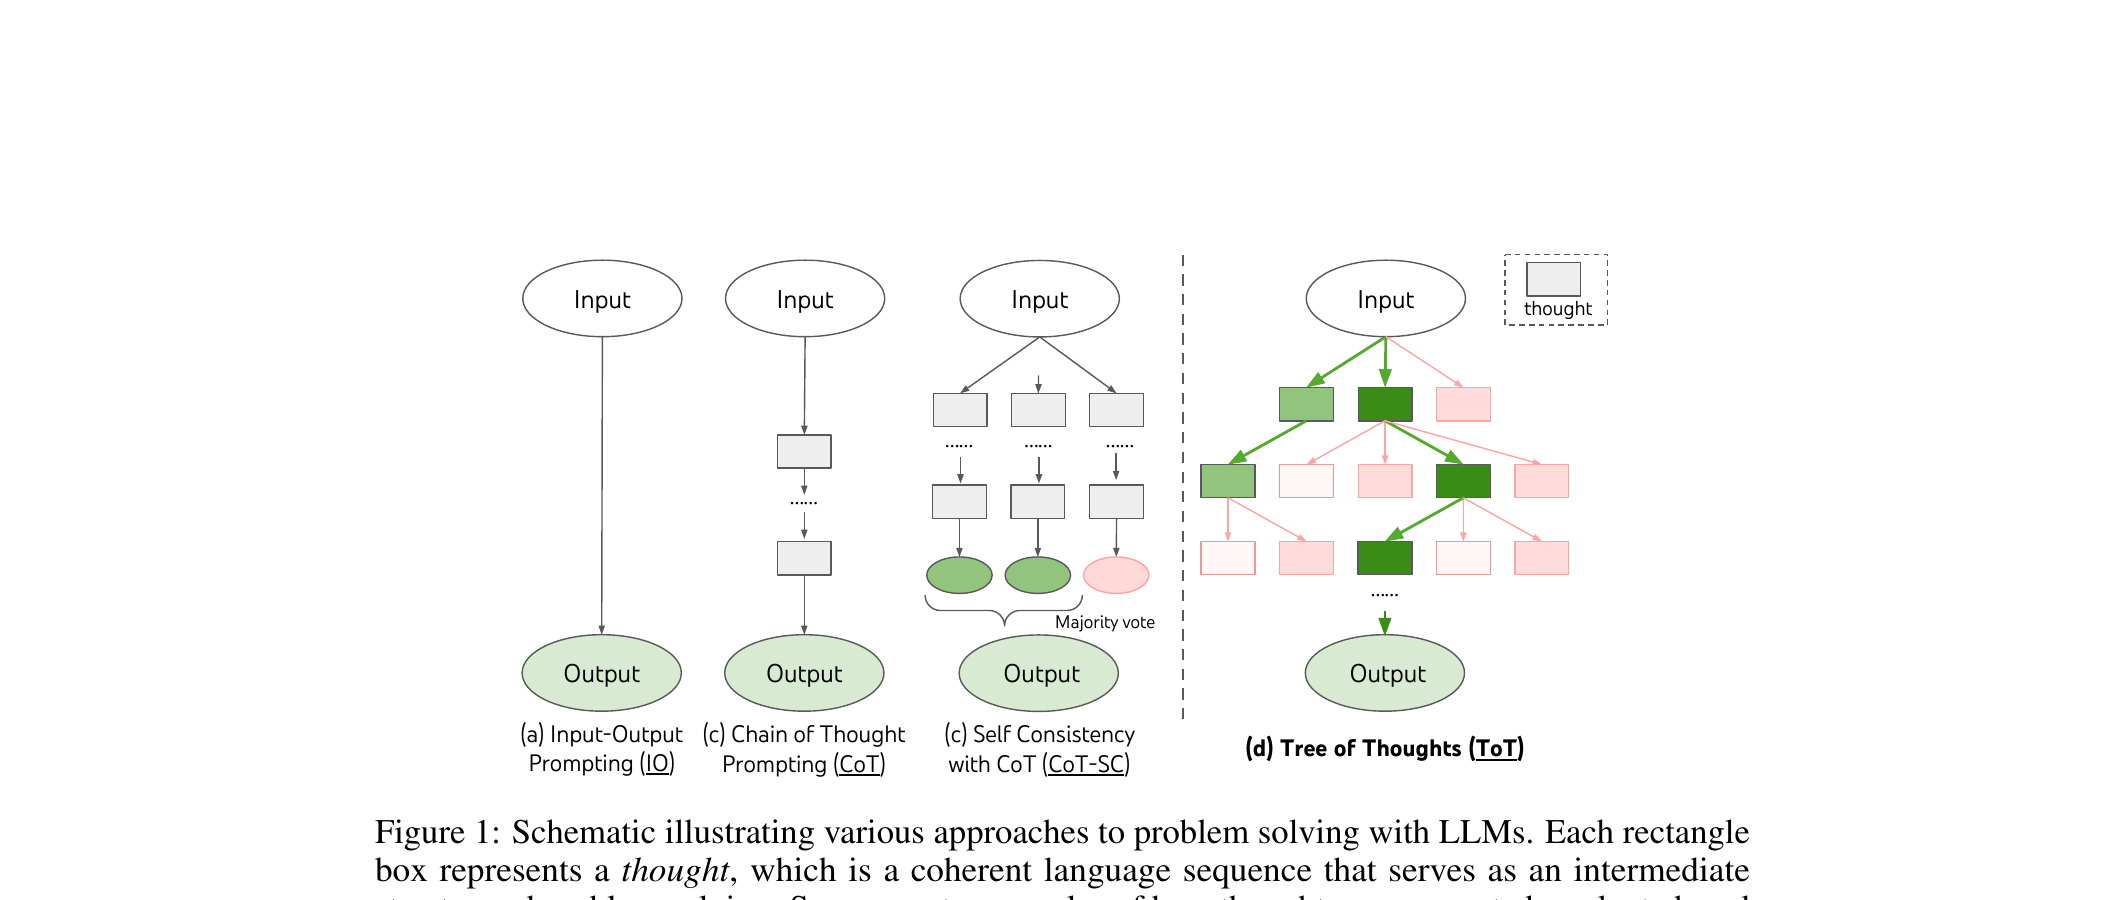
\includegraphics[width=0.9\textwidth]{fig-000.png}
    \caption*{\textbf{Original Figure 1.} (From~\cite{yao2023tot}.) Schematic illustrating IO, CoT, CoT-SC, and ToT approaches. ToT maintains a search tree over intermediate thoughts.}
\end{figure}

\begin{figure}[H]
    \centering
    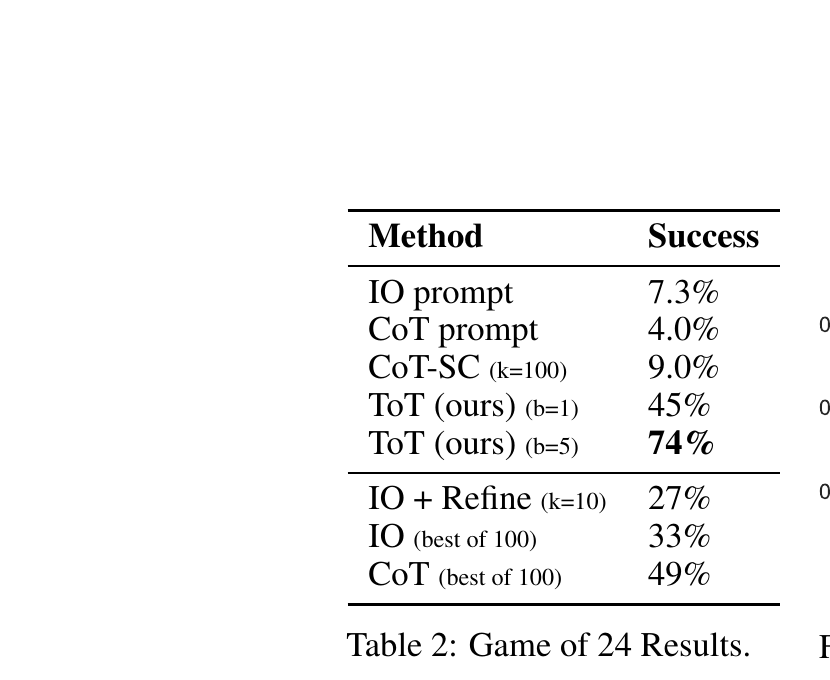
\includegraphics[width=0.7\textwidth]{fig-001.png}
    \caption*{\textbf{Original Table 2.} (From~\cite{yao2023tot}.) Game of 24 results with GPT-4. ToT ($b = 5$) achieves 74\%, far above IO (7.3\%) and CoT (4.0\%).}
\end{figure}

\begin{figure}[H]
    \centering
    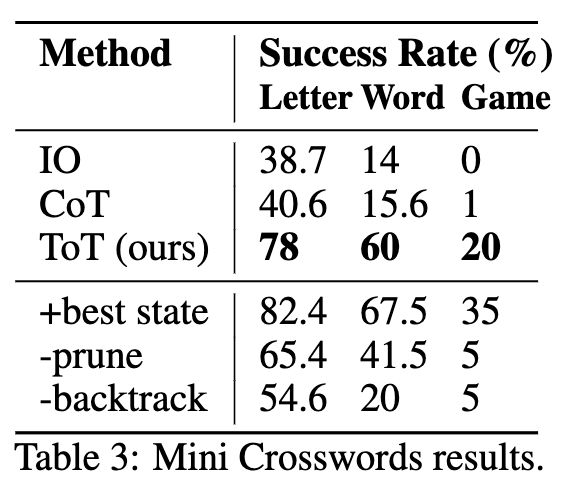
\includegraphics[width=0.7\textwidth]{fig-002.png}
    \caption*{\textbf{Original Table 3.} (From~\cite{yao2023tot}.) Mini Crosswords results with GPT-4. ToT achieves 78\% letter, 60\% word, and 20\% game accuracy.}
\end{figure}

\subsection*{Our Results}

\begin{figure}[H]
    \centering
    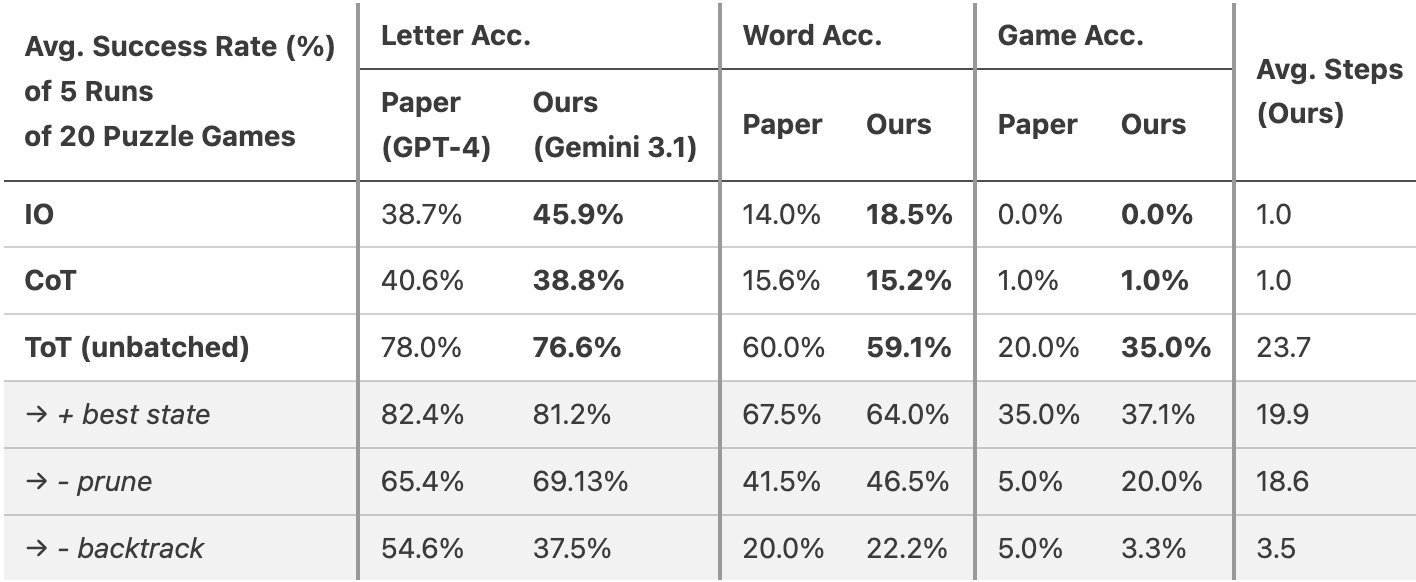
\includegraphics[width=0.85\textwidth]{fig-003.jpg}
    \caption{Game of 24 success rate ($n = 100$, $b = 5$). Unbatched ToT on both Gemini models exceeds GPT-4's 74\%. Batching collapses Gemini 2.5. The tiebreaker partially recovers it at zero cost.}
    \label{fig:game24_acc}
\end{figure}

\begin{table}[H]
    \centering
    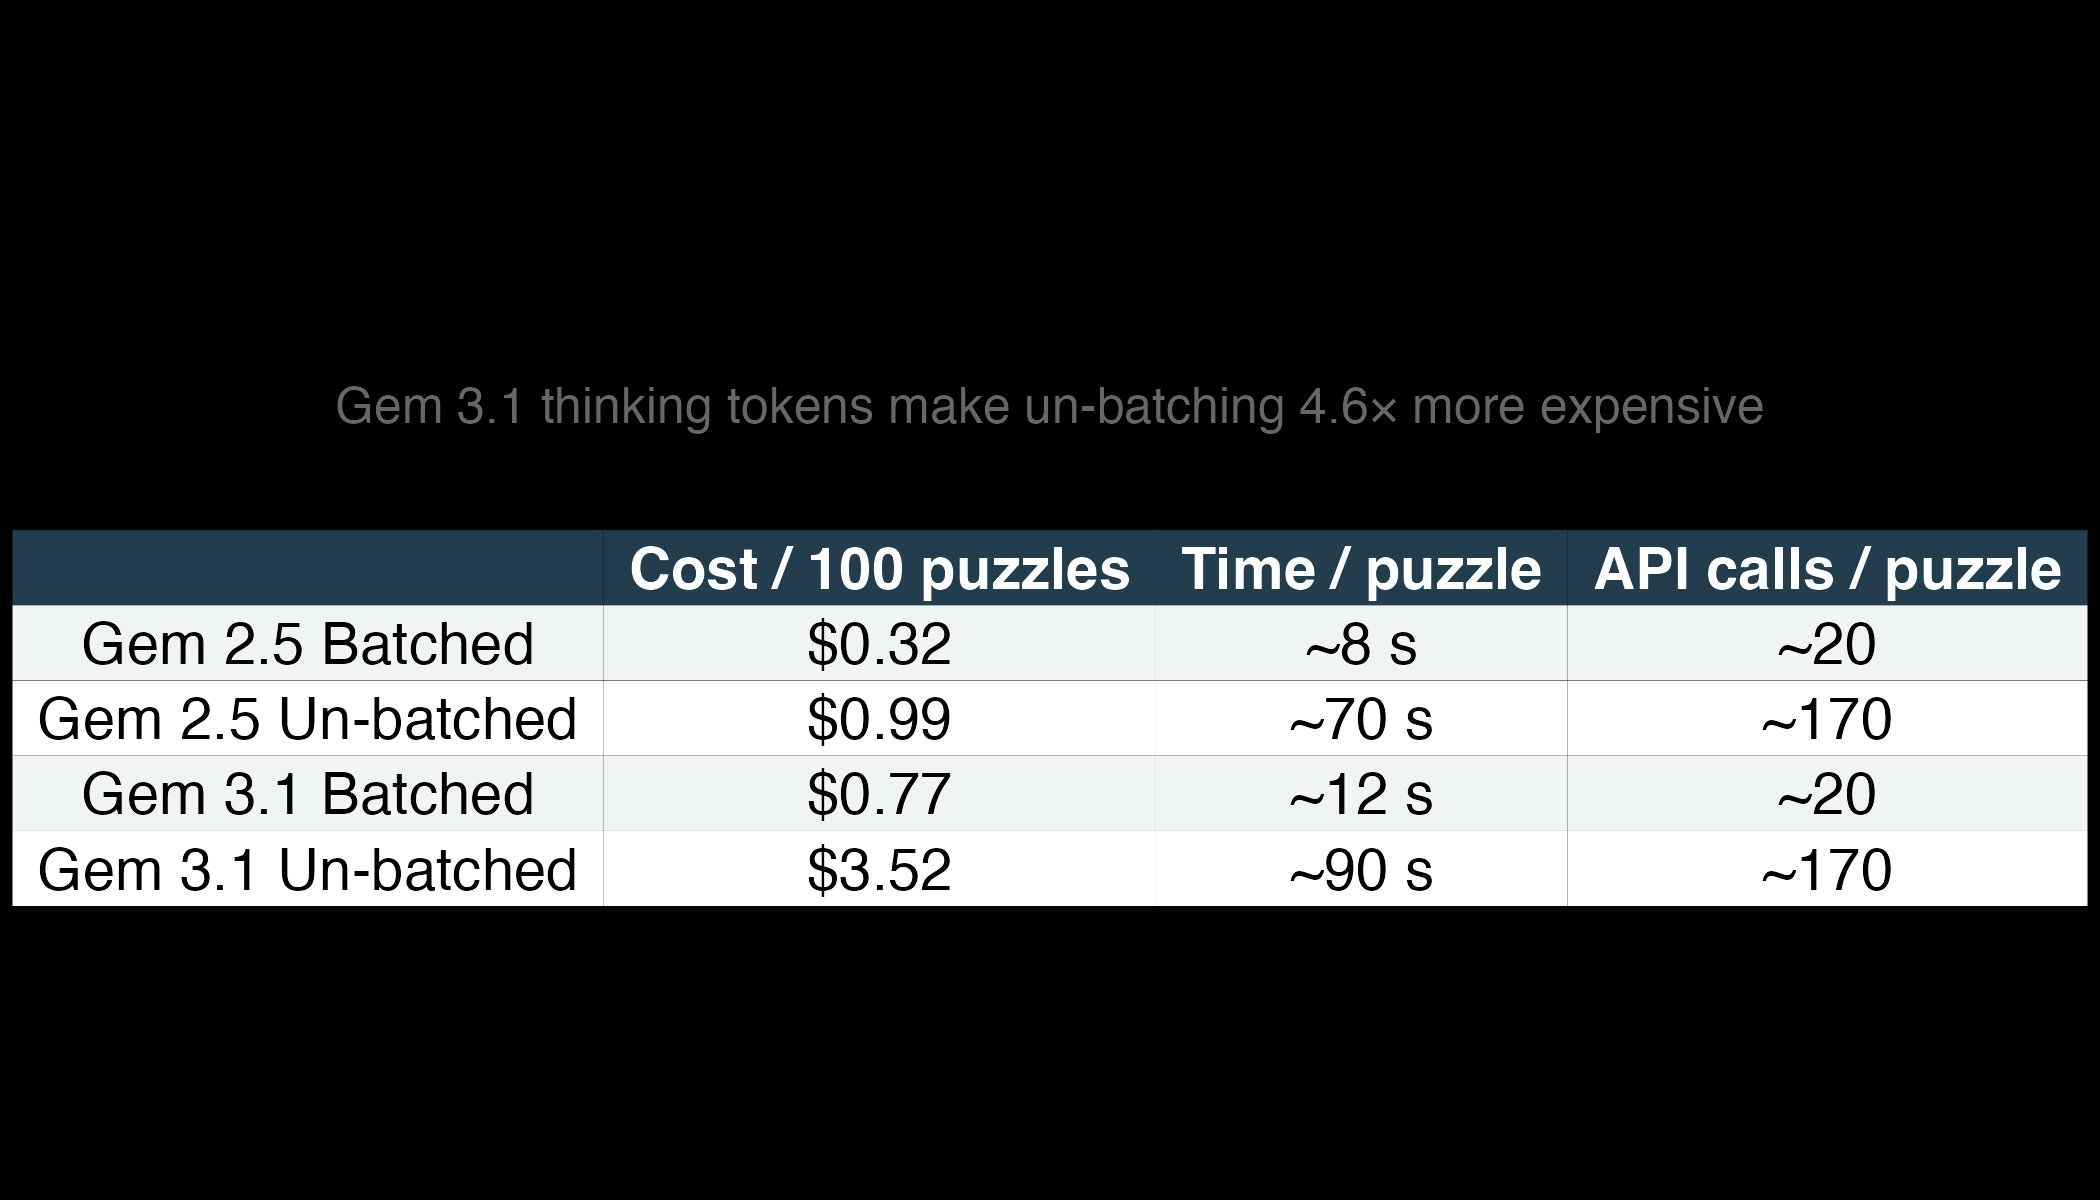
\includegraphics[width=0.7\textwidth]{fig-004.jpg}
    \caption{Cost of unbatching (ToT $b = 5$). Unbatching costs 3--4$\times$ more. Gemini 3.1 thinking tokens make it 4.6$\times$ more expensive.}
    \label{tab:cost}
\end{table}

\begin{figure}[H]
    \centering
    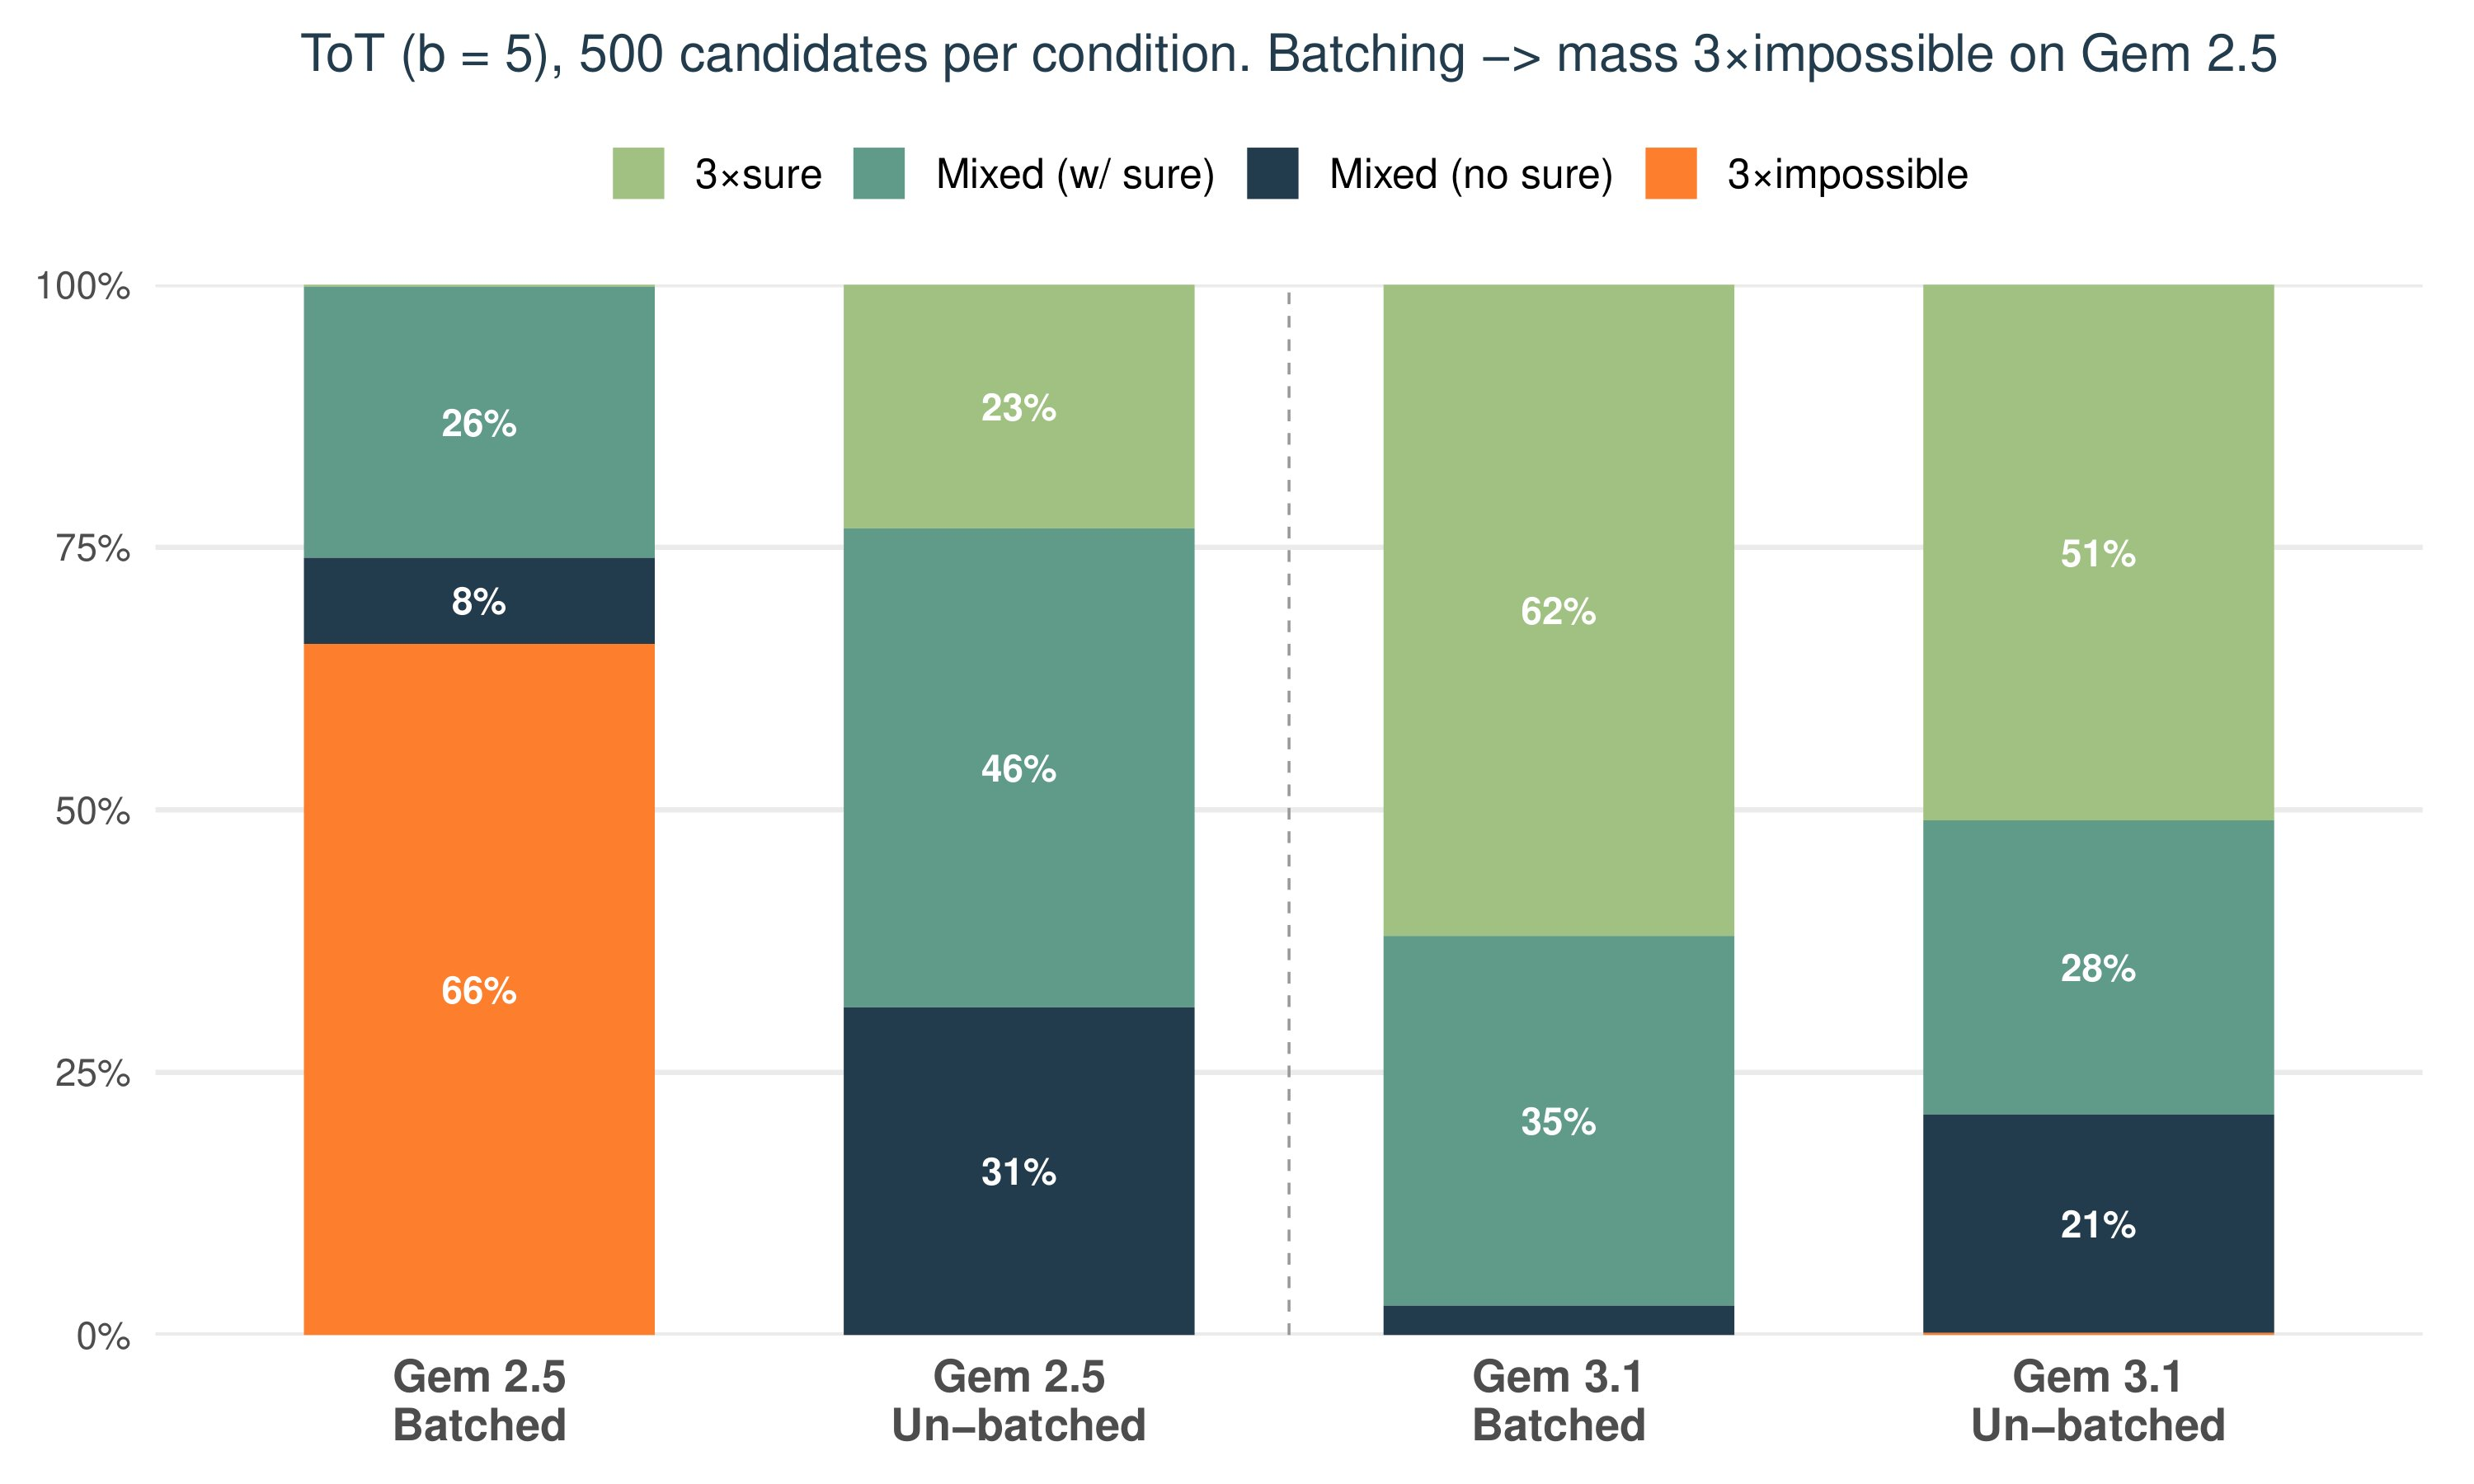
\includegraphics[width=0.85\textwidth]{fig-005.jpg}
    \caption{Evaluator verdict distribution at BFS depth 0 (500 candidates/condition). Batching causes Gemini 2.5 to vote ``impossible'' on 66\% of candidates (vs. 0\% unbatched). Gemini 3.1 resists: 62\% ``sure'' when batched.}
    \label{fig:verdict}
\end{figure}

\begin{table}[H]
    \centering
    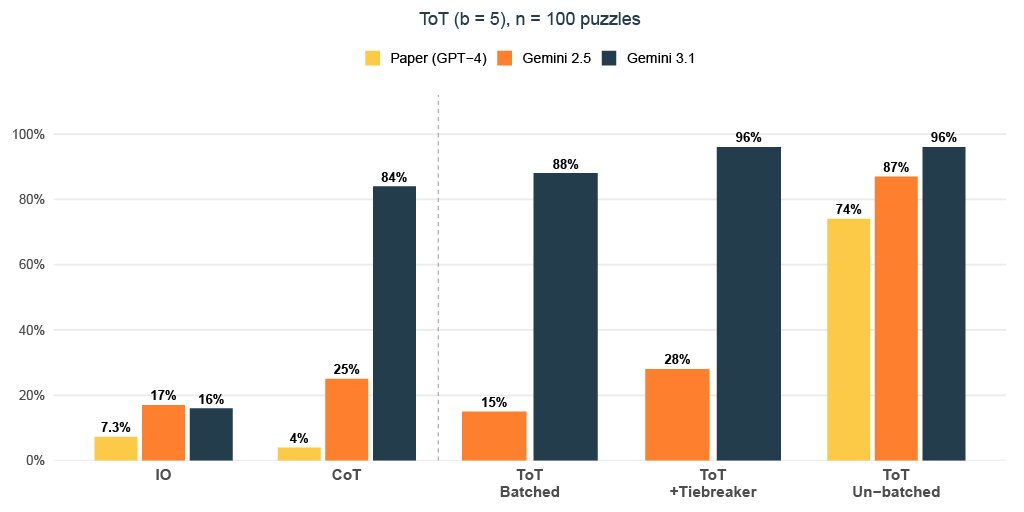
\includegraphics[width=0.85\textwidth]{fig-006.jpg}
    \caption{Mini Crosswords: average success rate (\%) over 5 runs of 20 puzzles. Gemini 3.1 matches or exceeds GPT-4.}
    \label{tab:crossword}
\end{table}

\begin{figure}[H]
    \centering
    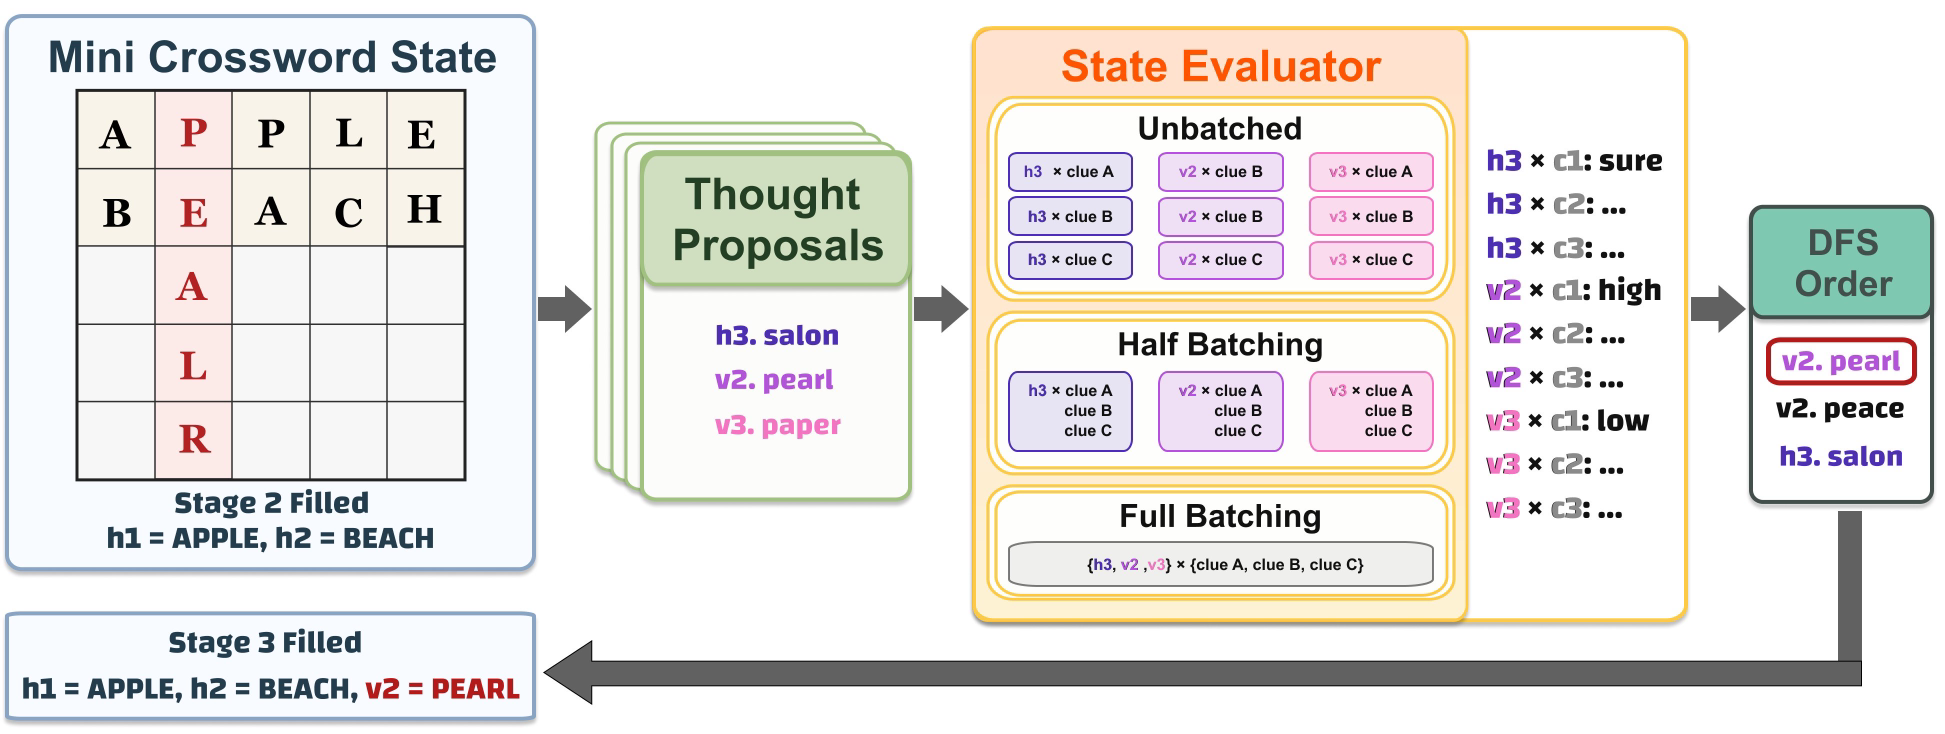
\includegraphics[width=0.85\textwidth]{fig-007.png}
    \caption{Crosswords batching schematic. Proposals are evaluated under three call shapes with decreasing cost but increasing list-position noise.}
    \label{fig:cw_schematic}
\end{figure}

\begin{figure}[H]
    \centering
    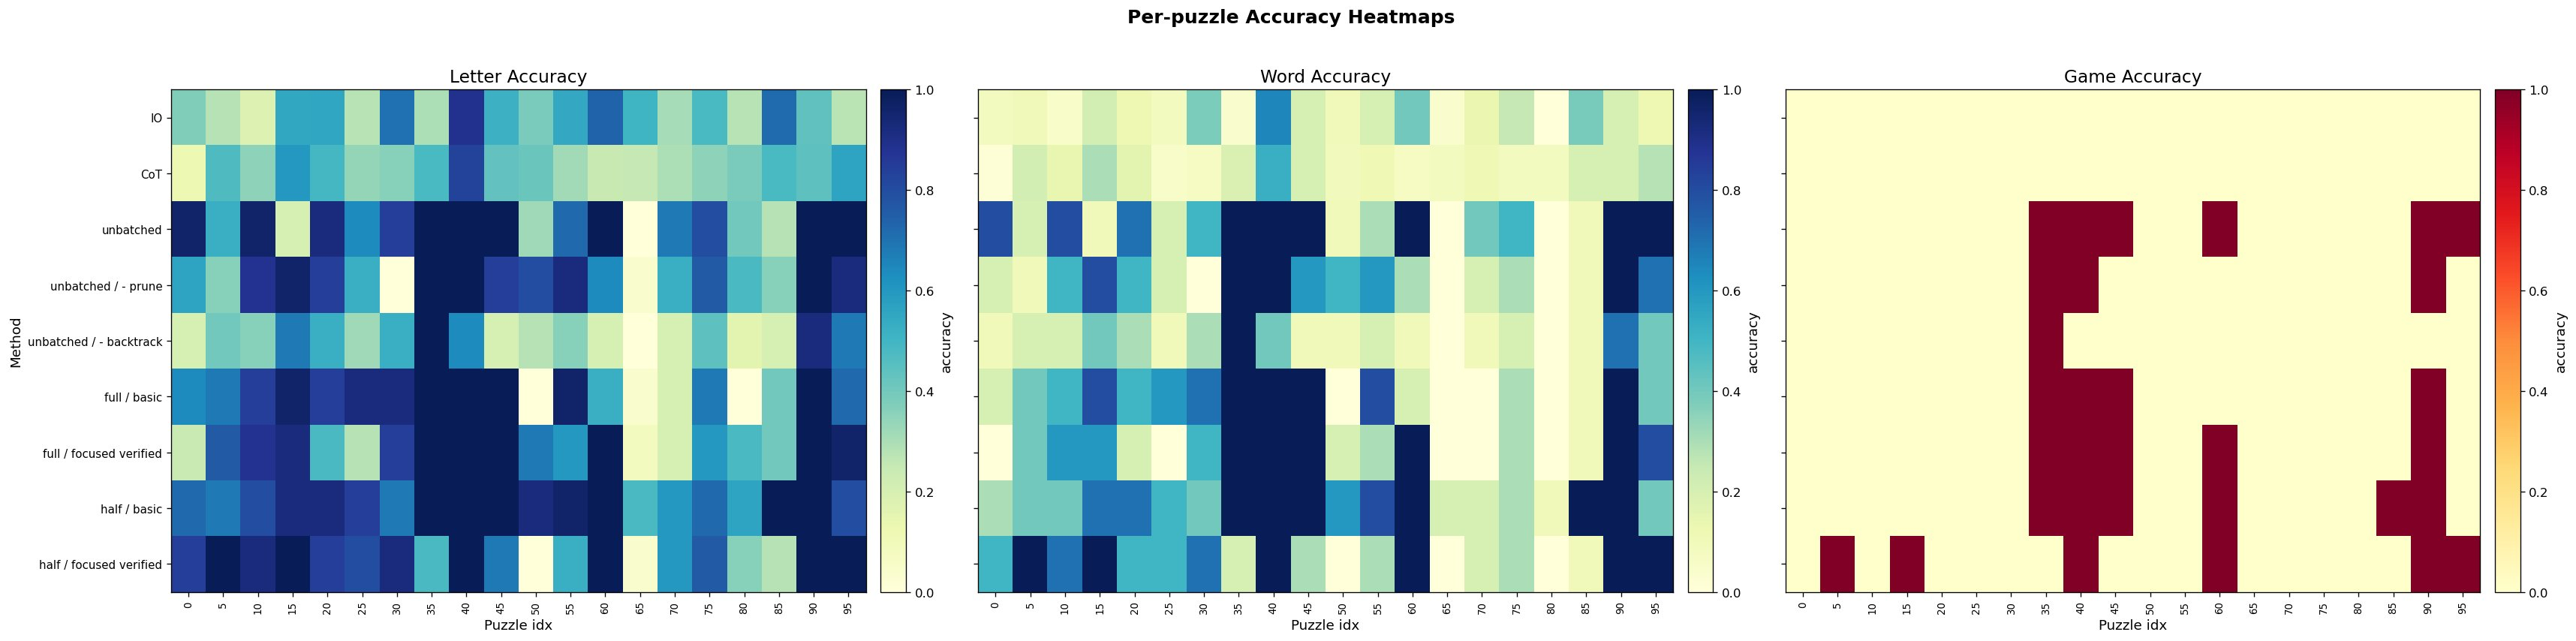
\includegraphics[width=0.85\textwidth]{fig-008.jpg}
    \caption{Per-puzzle accuracy heatmaps. Harder puzzles (idx 25--55) challenge all methods. ToT variants solve clusters IO/CoT cannot.}
    \label{fig:heatmap}
\end{figure}

\begin{figure}[H]
    \centering
    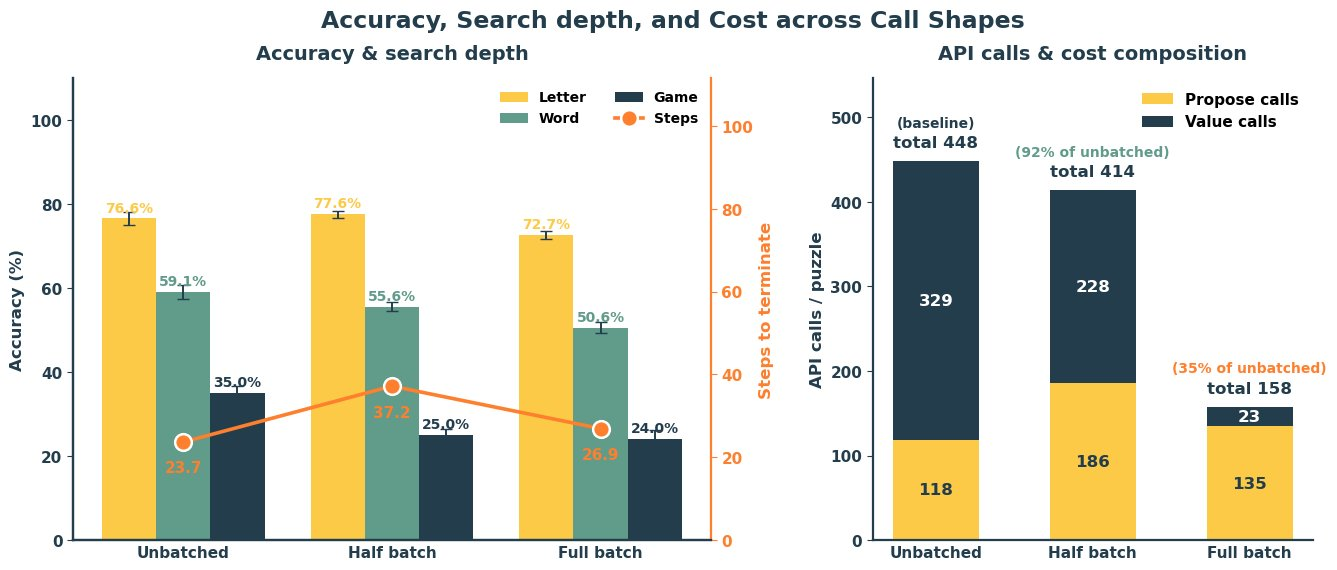
\includegraphics[width=0.85\textwidth]{fig-009.jpg}
    \caption{Accuracy, search depth, and cost across call shapes. Full batching cuts cost 65\% but drops game accuracy 35.0\% $\rightarrow$ 24.0\%. Half batching achieves the highest letter accuracy (77.6\%).}
    \label{fig:cw_batch}
\end{figure}

\begin{figure}[H]
    \centering
    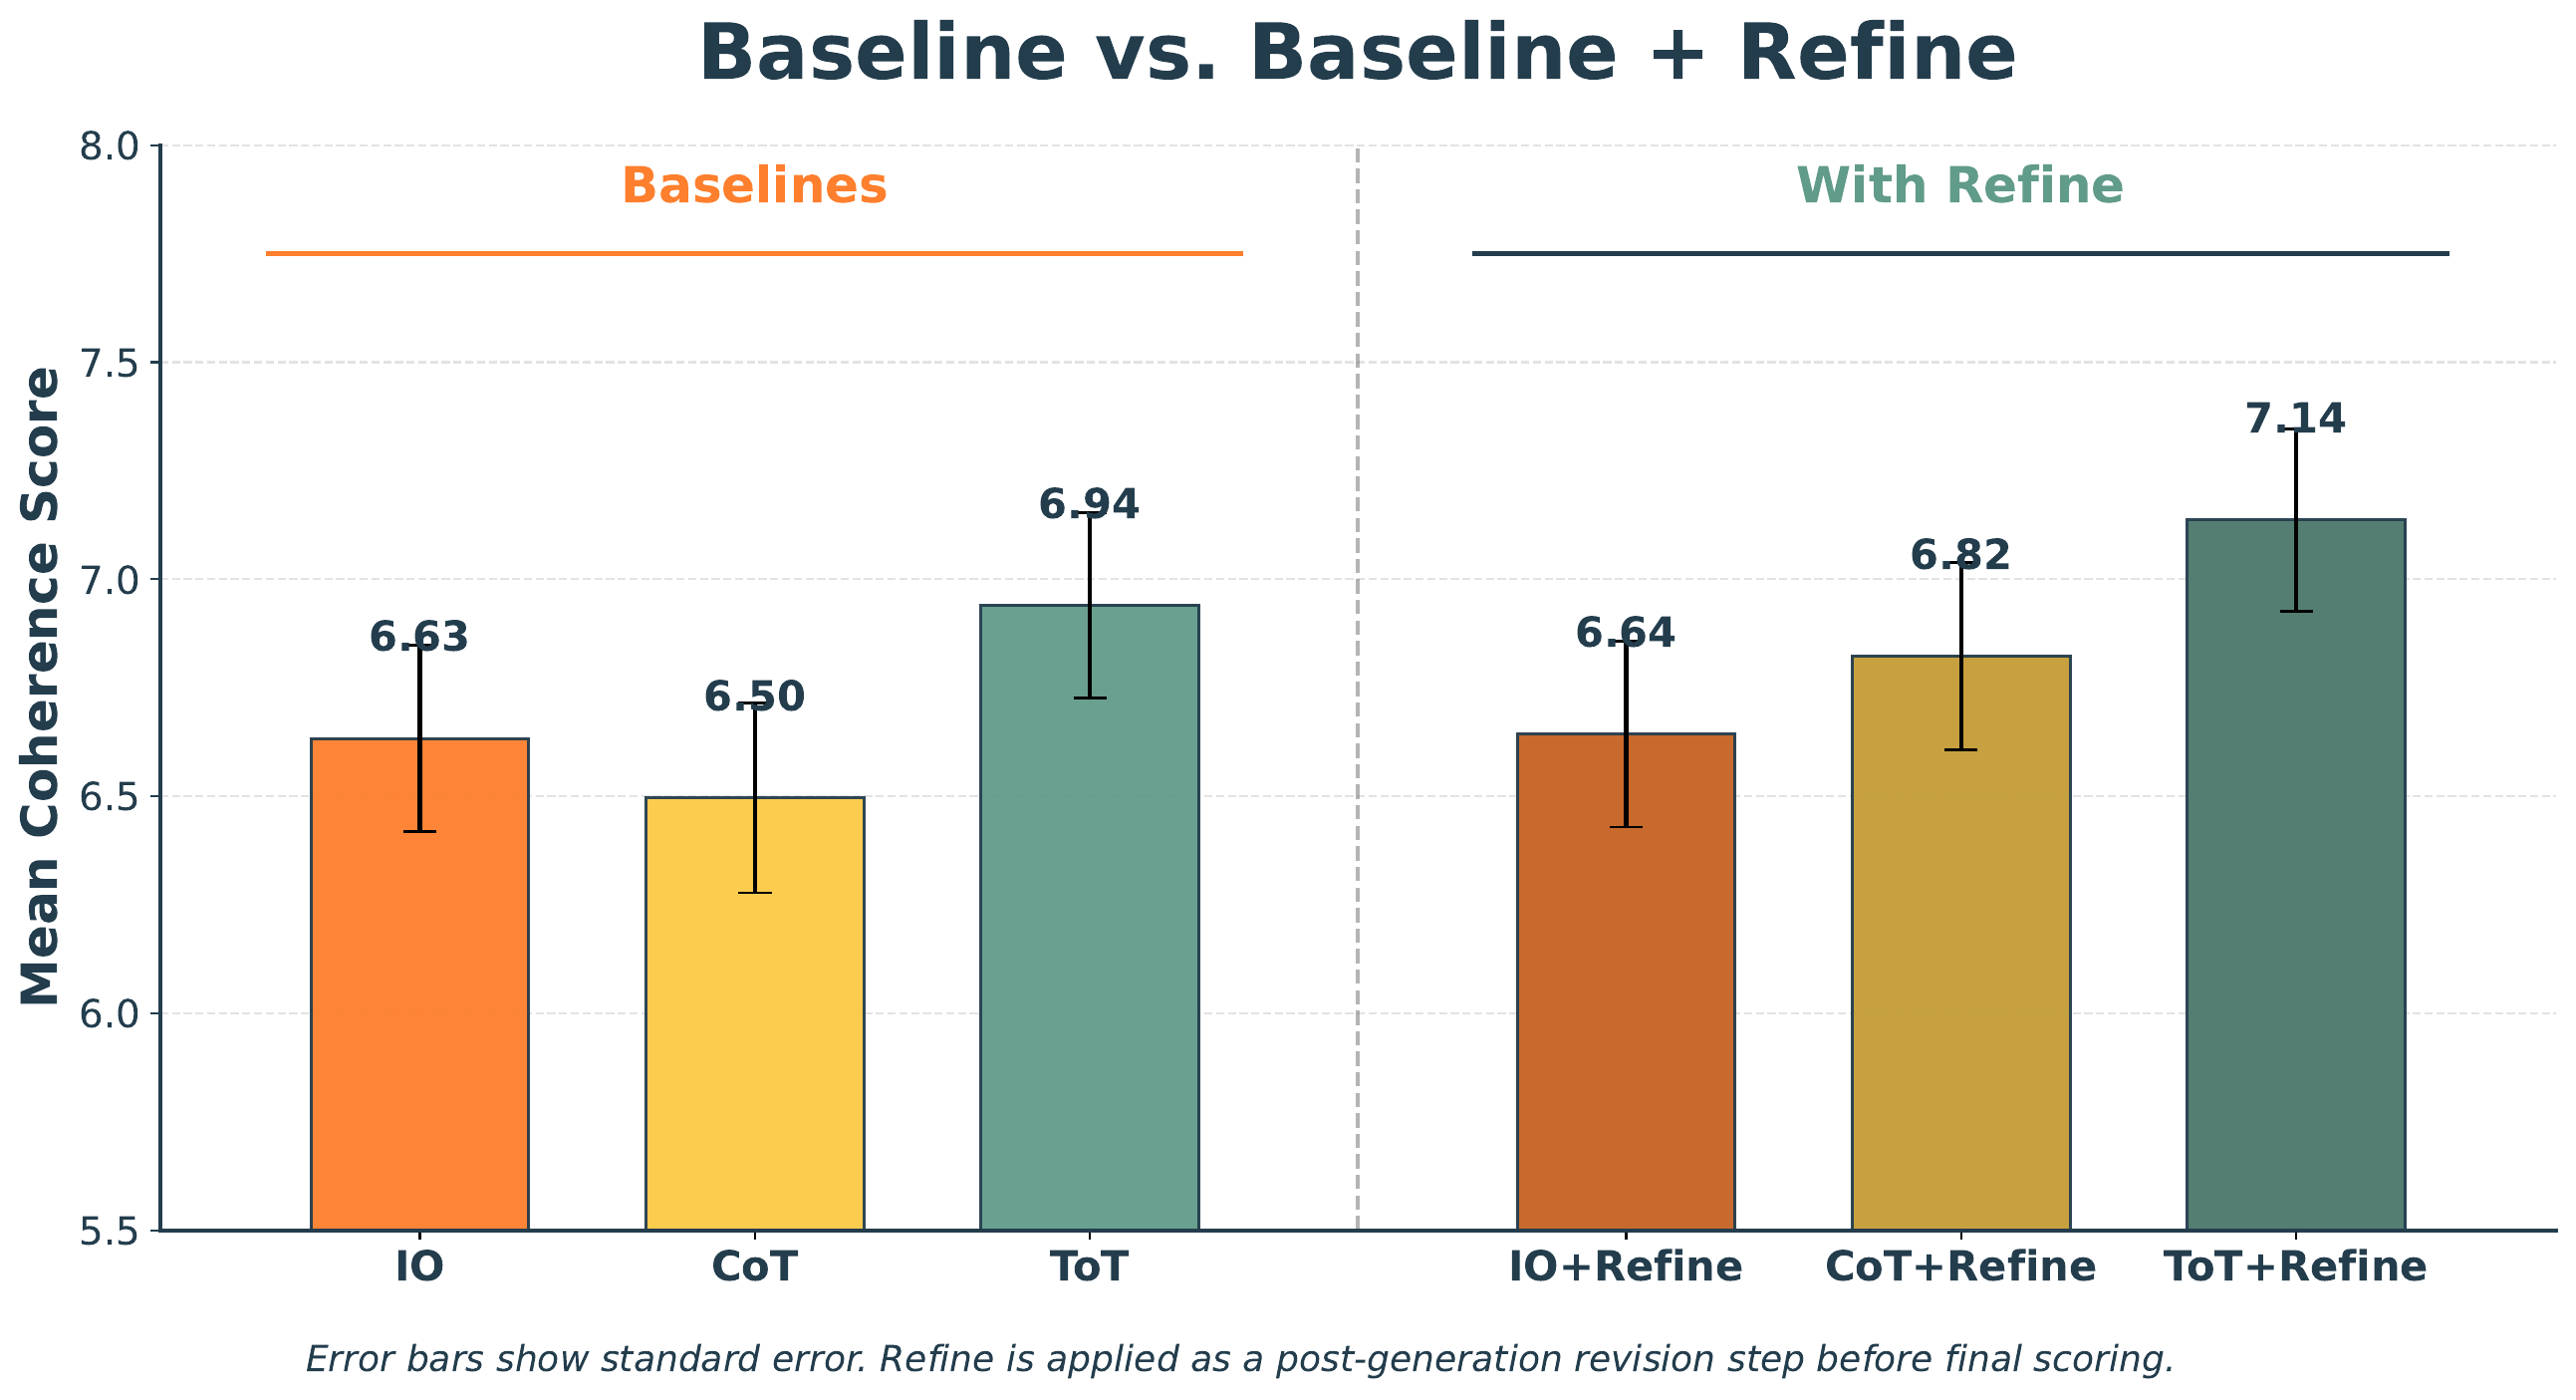
\includegraphics[width=0.85\textwidth]{fig-010.png}
    \caption{Baseline vs. Baseline + Refine. Refinement modestly improves all methods. ToT+Refine achieves 7.14.}
    \label{fig:cw_baseline}
\end{figure}

\begin{figure}[H]
    \centering
    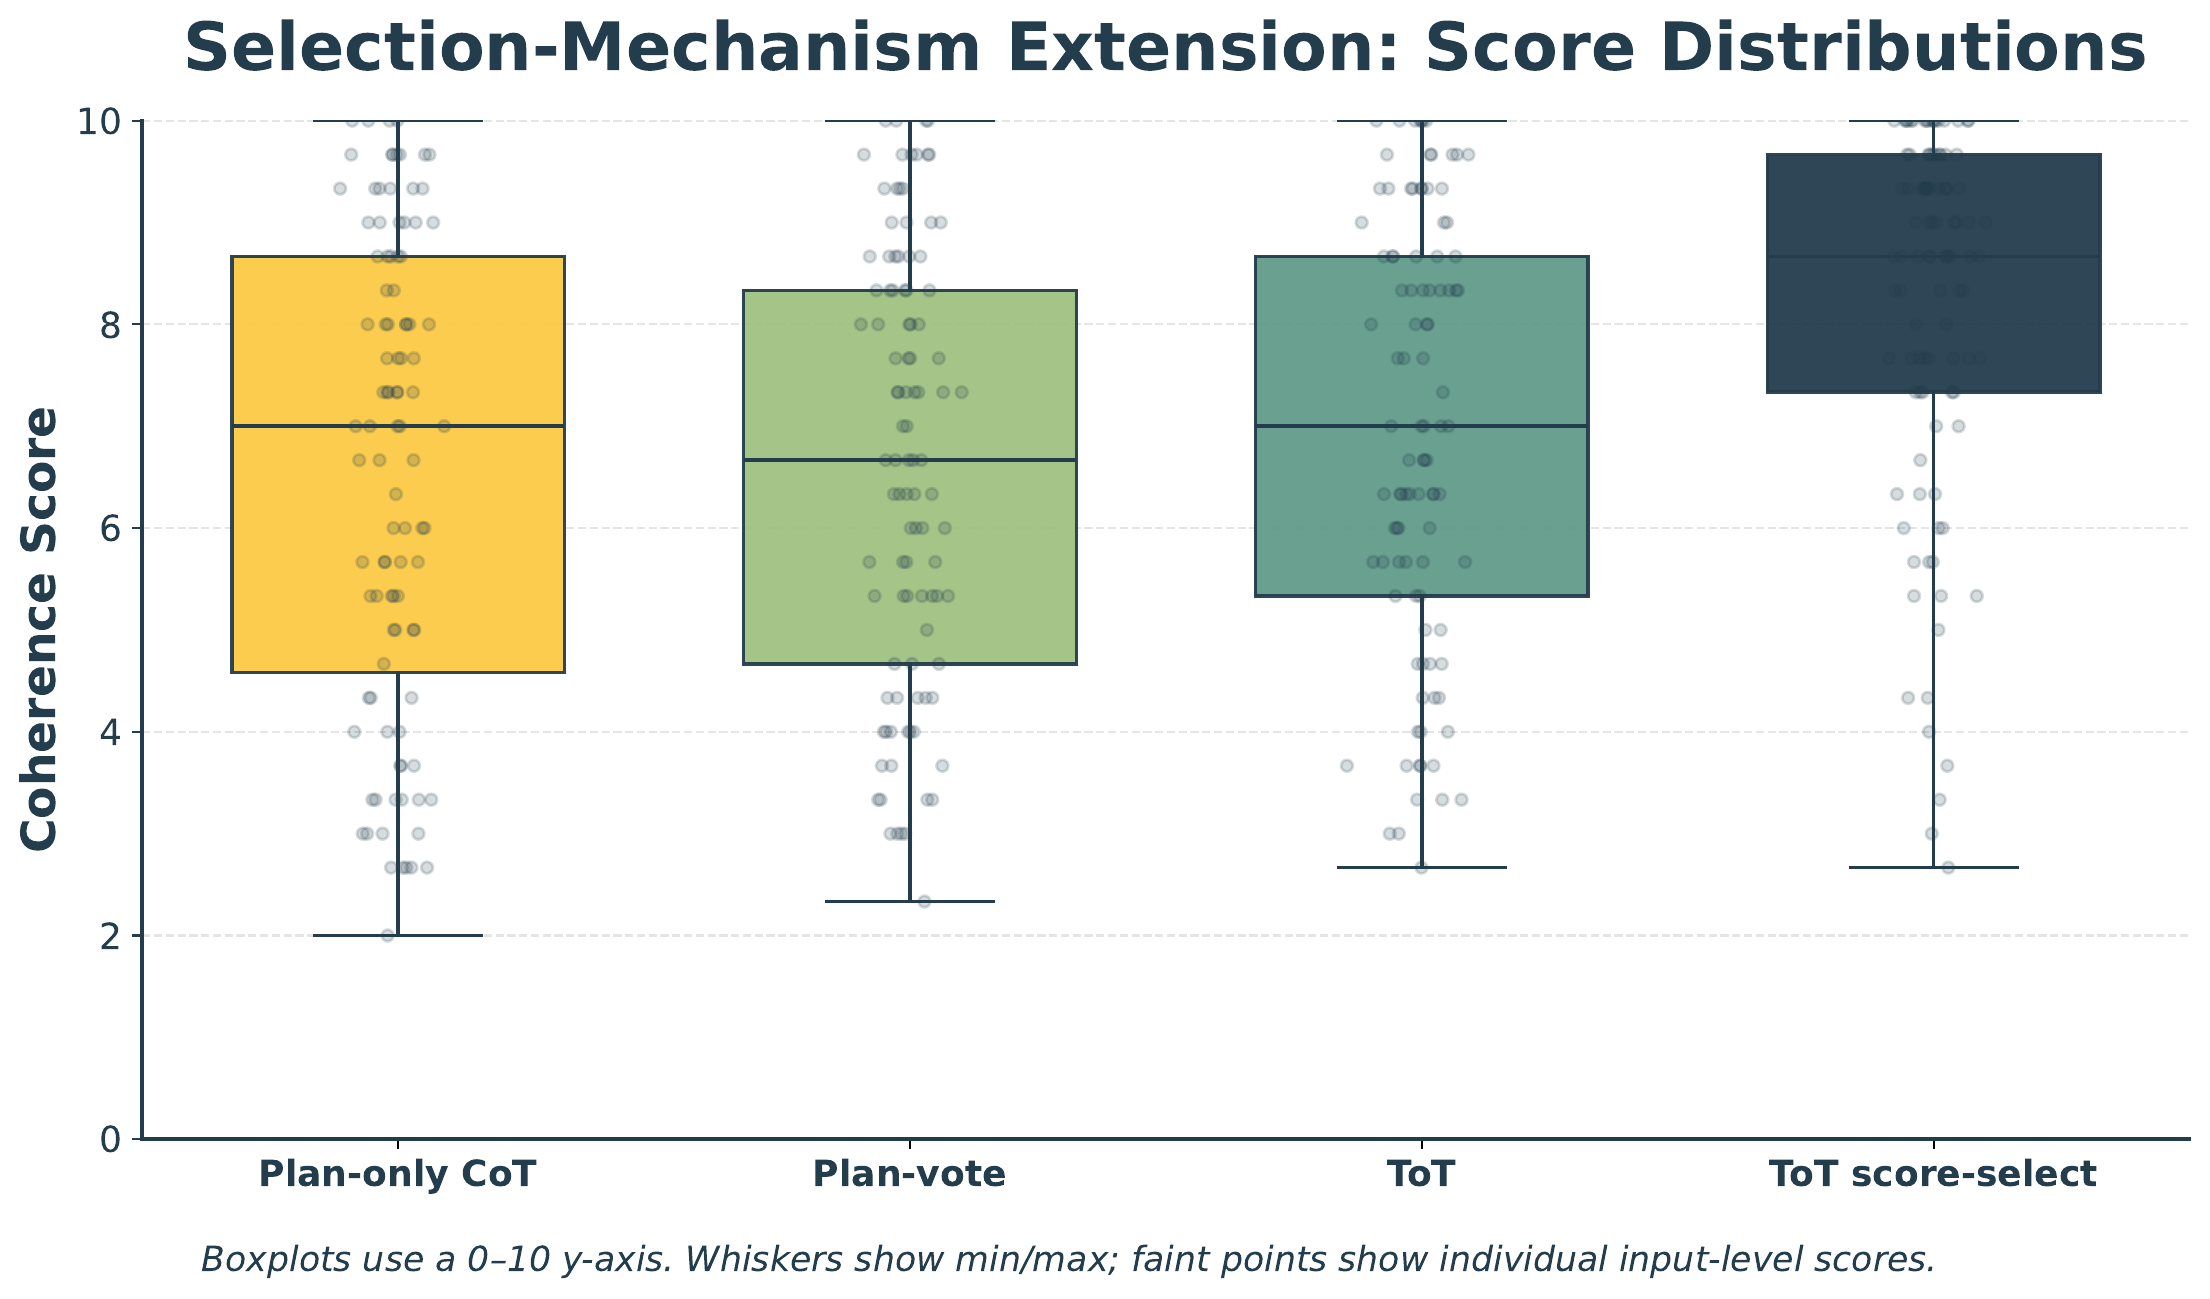
\includegraphics[width=0.85\textwidth]{fig-011.png}
    \caption{Selection-mechanism ablations. Score-select concentrates scores near the top. Standard ToT has the widest spread.}
    \label{fig:cw_select}
\end{figure}

\begin{figure}[H]
    \centering
    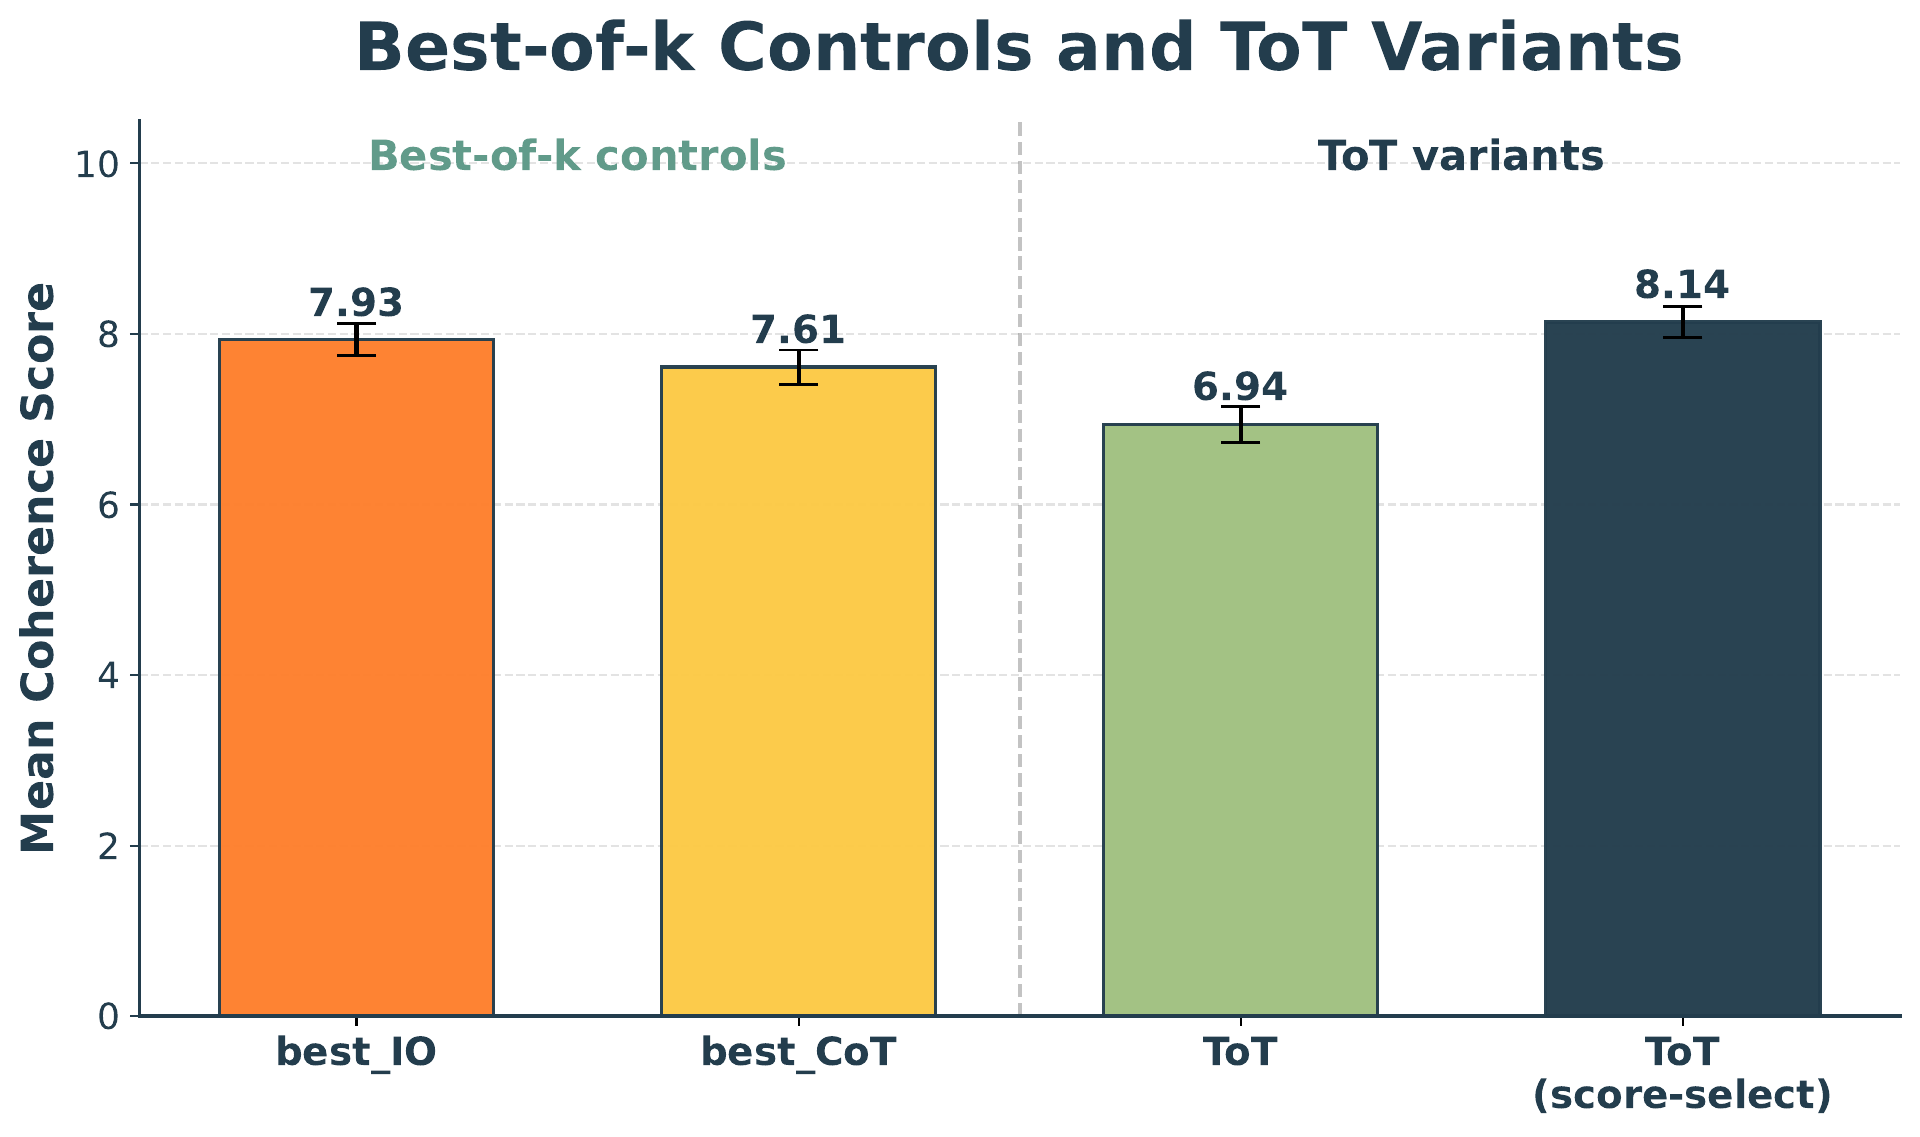
\includegraphics[width=0.85\textwidth]{fig-012.png}
    \caption{Best-of-k controls vs. ToT variants. Best-of-k IO (7.93) and ToT score-select (8.14) both outperform vote-based ToT (6.94).}
    \label{fig:cw_bestofk}
\end{figure}

\clearpage
\begin{thebibliography}{9}

\bibitem{yao2023tot}
S. Yao et al., ``Tree of Thoughts: Deliberate Problem Solving with Large Language Models,'' \textit{NeurIPS}, 2023.

\bibitem{wei2022cot}
J. Wei et al., ``Chain-of-Thought Prompting Elicits Reasoning in Large Language Models,'' \textit{NeurIPS}, 2022.

\bibitem{cheng2023batch}
Z. Cheng et al., ``Batch Prompting: Efficient Inference with LLM APIs,'' \textit{EMNLP Industry Track}, 2023.

\bibitem{lin2024batchprompt}
J. Lin et al., ``BatchPrompt: Accomplish More with Less,'' \textit{ICLR}, 2024.

\bibitem{lee2022coauthor}
M. Lee, P. Liang, \& Q. Yang, ``CoAuthor: Designing a Human-AI Collaborative Writing Dataset,'' \textit{CHI}, 2022.

\bibitem{tot_code}
ToT reference code: \url{https://github.com/princeton-nlp/tree-of-thought-llm}

\bibitem{puzzle_data}
Puzzle data: 4nums.com (Game of 24), GooBix (Crosswords), randomwordgenerator.com (Creative Writing).

\bibitem{vertexai}
Google Cloud Vertex AI (Gemini 2.5 Flash-Lite, Gemini 3.1 Flash-Lite Preview).

\bibitem{sympy}
SymPy: symbolic mathematics library for Python.

\end{thebibliography}

\end{document}
